\documentclass[11pt]{article}

\usepackage{deauthor}
\usepackage{times}
\usepackage{authblk}

%\usepackage{amsthm,amsmath,amssymb,amsfonts}
%\usepackage[inline]{enumitem}
\usepackage{caption,subcaption}
\usepackage{balance}
%\usepackage[binary-units]{siunitx}
\usepackage{graphicx}
\usepackage{hyperref}


%% Comments
\newcommand{\mo}[1]{{\color{red} #1}}
\newcommand{\sajjad}[1]{{\color{green} #1}}


%% Replicas.
\newcommand{\Service}{\mathcal{S}}
\newcommand{\Replicas}{\mathcal{R}}
\newcommand{\Miners}{\mathcal{M}}
\newcommand{\Clients}{\mathcal{C}}
\newcommand{\Faulty}{\mathcal{F}}
\newcommand{\NonFaulty}{\mathcal{NF}}
\newcommand{\n}[1]{\mathbf{n}_{#1}}
\newcommand{\f}[1]{\mathbf{f}_{#1}}
\newcommand{\CC}{\mathbf{c}}
\newcommand{\ID}[1]{\mathop{\textsf{id}}(#1)}
\newcommand{\Replica}[1][r]{\textsc{#1}}
\newcommand{\Primary}[1][p]{\textsc{#1}}
\newcommand{\Miner}[1][m]{\textsc{#1}}
\newcommand{\Client}[1][c]{\MakeLowercase{#1}}

%% Special names.
\newcommand{\MName}[1]{\textsc{#1}}
\newcommand{\Name}[1]{\texttt{#1}}
\newcommand{\BFT}{\textsc{bft}}
\newcommand{\PoW}{\textsc{PoW}}
\newcommand{\PoC}{\textsc{PoC}}
\newcommand{\PoCf}{\textsc{Power-of-Collaboration}}
\newcommand{\DualChain}{\textsc{HybridChain}}
\newcommand{\ZZ}{\textsc{Zyzzyva}}
\newcommand{\PoE}{\textsc{PoE}}
\newcommand{\PBFT}{\textsc{Pbft}}
\newcommand{\pbft}{\textsc{Pbft}}
\newcommand{\hotstuff}{\textsc{HotStuff}}
\newcommand{\SBFT}{\textsc{SBFT}}
\newcommand{\ResDB}{\textsc{ResilientDB}}
\newcommand{\MAC}{\textsc{Mac}}
\newcommand{\DS}{\textsc{DS}}


\newcommand{\View}[1][v]{#1}


%PoC names
\newcommand{\Bitcoin}{\MName{Bitcoin}}
\newcommand{\Ethereum}{\Name{Ethereum}}
\newcommand{\blockchains}{\MName{blockchains}}
\newcommand{\block}{\mathfrak{B}}

\newcommand{\NET}[1][NET]{\textsc{#1}}
\newcommand{\Slice}[1]{\mathcal{S}_{#1}}
\newcommand{\Sequence}{\textsc{Seq}}
\newcommand{\TXNBlock}{\textsc{TB}}

\newcommand{\Digest}[1]{\MName{Digest}(#1)}
\newcommand{\BBlock}{\mathbb{B}}
\newcommand{\Checksum}[2]{\mathop{\textnormal{\texttt{checksum}}_{#2}}(#1)}


%% PoC protocol.
\newcommand{\Certificate}{\mathfrak{C}}
\newcommand{\T}{\tau}
\newcommand{\Transaction}[1][t]{\MakeUppercase{#1}}
\newcommand{\Message}[2]{\textsc{#1}(#2)}
\newcommand{\SignMessage}[2]{\langle#1\rangle_{#2}}
\newcommand{\SignShare}[2]{s\langle#1\rangle_{#2}}
\newcommand{\Hash}[1]{\texttt{hash}(#1)}
\newcommand{\Supported}[4]{\texttt{Support}_{#1}(#2, #3, #4)}
\newcommand{\ViewCommitted}[4]{\texttt{VCommit}_{#1}(#2, #3, #4)}
\newcommand{\Executed}[4]{\texttt{Execute}_{#1}(#2, #3, #4)}
\newcommand{\SliceShifting}{\MName{SliceShifting}}
\newcommand{\ShiftRound}{\MName{SR}}


%% Misc.
\newcommand{\True}{\texttt{true}}
\newcommand{\False}{\texttt{false}}
\newcommand{\abs}[1]{\lvert #1 \rvert}
\newcommand{\union}{\cup}
\newcommand{\intersect}{\cap}
\newcommand{\difference}{\setminus}
\newcommand{\BigO}[1]{\mathcal{O}(#1)}
\newcommand{\BigOm}[1]{\Omega(#1)}

%\newtheorem{theorem}{Theorem}
%\newtheorem{definition}[theorem]{Definition}
%\newtheorem{proposition}[theorem]{Proposition}
%\newtheorem{example}[theorem]{Example}
%\newtheorem{corollary}[theorem]{Corollary}

%% myprotocol
\usepackage{algorithmic}
\newcommand{\GETS}{:=}
\newenvironment{myprotocol}{
    \hrule
    \smallskip
    \footnotesize
    \algsetup{linenosize=\footnotesize}
    \begin{algorithmic}[1]
        \newcommand{\SPACE}{\item[]}
        \newcommand{\TITLE}[2]{\item[] \textbf{\underline{##1}} (##2) \textbf{:}\\[2pt]}
        \makeatletter
            \newcommand{\EVENT}[1]{\STATE \textbf{event} ##1 \textbf{do}}
            \newcommand{\ENDEVENT}{ \STATE \textbf{end event}}
        \makeatother
}{
    \end{algorithmic}
    \smallskip
    \hrule
}

%% common
\usepackage{amsfonts,amssymb, amsmath, colortbl, makecell}
%\usepackage[table]{xcolor}


%% PGF/TikZ setup for figures and plots.
\usepackage{tikz,pgfplots,pgfplotstable}
\usetikzlibrary{arrows.meta,calc,decorations.pathreplacing,patterns,shapes}
\tikzset{
    dot/.append style={circle,scale=0.35,draw=black,fill=black},
    sdot/.append style={scale=0.45,draw=black,fill=black},
    label/.append style={align=center,font=\strut\footnotesize},
    >=Stealth,
    every edge/.append style={semithick},
    thread/.append style={align=center,draw,thick,rectangle,text width=1cm,text height=2ex,text depth=.25ex,minimum height=0.75cm,font=\strut},
}

% Seven colors safe for use color blindness.
% Colors taken from doi:10.1038/nmeth.1618. 
\definecolor{colA}{RGB}{230,159,0}
\definecolor{colB}{RGB}{86,180,233}
\definecolor{colC}{RGB}{0,158,115}
\definecolor{colD}{RGB}{240,228,66}
\definecolor{colE}{RGB}{0,114,178}
\definecolor{colF}{RGB}{213,94,0}
\definecolor{colG}{RGB}{204,121,167}
\definecolor{colH}{RGB}{238,130,238}
\definecolor{colI}{RGB}{64,224,208}
\definecolor{colGrey}{RGB}{211,211,211}
\definecolor{colIvory}{RGB}{255,235,215}
\definecolor{colDeepPink}{RGB}{255,20,147}
\definecolor{colLightRed}{RGB}{255,235,0}

%% Cycle list for evaluation graphs.
\pgfplotscreateplotcyclelist{mycyclelist}{
    very thick,solid,black,every mark/.append style={solid},mark=*\\         %PoE
    very thick,solid,colG,every mark/.append style={solid},mark=*\\          %PBFT
    very thick,solid,colB,every mark/.append style={solid},mark=*\\          %ZZ
    very thick,solid,colE,every mark/.append style={solid},mark=*\\          %SBFT
    very thick,solid,colD,every mark/.append style={solid},mark=*\\          %HS
}


%% Make-up for evaluation graphs.
\pgfplotsset{
    compat=1.16,
    width=195pt,
    height=156pt,
    every axis title shift=0pt,
    max space between ticks=25,
    every axis/.append style={
        cycle list name=mycyclelist,
        ymin=0,
        enlargelimits=0.05,
        scale ticks above exponent=1,
        scaled x ticks=false,
        xtick=data,
        mark size=1pt,
        font=\Large,
        y tick label style={
            /pgf/number format/precision=1,
            /pgf/number format/fixed,
            /pgf/number format/fixed zerofill
        },
        ylabel shift={-5pt}
    },
    every axis legend/.append style={
        cells={anchor=west}
    }
}

%% Plot-style for tikzpictures.
\tikzset{
   plot/.append style={baseline,scale=0.65}
}


%% Figures and plots.
\usepackage{tikz,pgfplots,pgfplotstable}
\usetikzlibrary{arrows.meta}
\tikzset{
    >=Stealth,
    dot/.style={circle,scale=0.35,draw=black,fill=black},
    node_text/.append style={font=\strut\bfseries},
    plot/.append style={baseline,scale=0.8},
    label/.append style={font=\strut\footnotesize}
}
\pgfplotscreateplotcyclelist{mycyclelist}{
    thick,black   ,every mark/.append style={solid,fill=\pgfplotsmarklistfill},mark=*\\ 
    thick,red     ,every mark/.append style={solid,fill=\pgfplotsmarklistfill},mark=square*\\
    thick,blue    ,every mark/.append style={solid,fill=\pgfplotsmarklistfill},mark=triangle*\\
    thick,teal    ,every mark/.append style={solid,fill=\pgfplotsmarklistfill},mark=pentagon*\\
    thick,brown   ,every mark/.append style={solid,fill=\pgfplotsmarklistfill},mark=halfsquare*\\ 
    thick,orange  ,every mark/.append style={solid,fill=\pgfplotsmarklistfill},mark=halfcircle*\\
    thick,violet  ,every mark/.append style={solid,fill=\pgfplotsmarklistfill,rotate=180},mark=halfdiamond*\\
}
\pgfplotscreateplotcyclelist{mycyclelistex}{
    black   ,every mark/.append style={solid,fill=\pgfplotsmarklistfill},mark=*\\ 
    red     ,every mark/.append style={solid,fill=\pgfplotsmarklistfill},mark=square*\\
}

\pgfplotsset{
    % tick label style={font=\Large},
    % legend style={font=\LARGE,cells={anchor=west}},
    % title style={font=\Large},
    % label style={font=\LARGE},
    % width=262.5pt,
    % height=185pt,
    scaled y ticks = false,
    every axis/.append style={
        ylabel near ticks,
        xlabel near ticks,
        mark size=2.5pt,
        cycle list name=mycyclelist,
        % font=\Large,
        y tick label style={
                        /pgf/number format/precision=1,
                        /pgf/number format/fixed,
                        /pgf/number format/fixed zerofill
                    }
    },
    barstyle/.append style={
        ybar,
        bar width={0.5cm},
        enlarge x limits=0.4,
        enlarge y limits={upper=0.025},
        ymin=0,
        xtick=data
    }
    every axis/.append style={
        ylabel near ticks,
        xlabel near ticks,
        mark size=1pt,
        cycle list name=mycyclelist,
        % font=\Large,
        enlargelimits=0.1
    },
}

\newcommand{\resultgraph}[6]{\begin{tikzpicture}[plot]
        \begin{axis}[xlabel={#3},ylabel={#4}, title={#2},
            xticklabels={#6},
            %xticklabels={32,64,128,256,512},
            %xtick={8,9,10,11,12},
            %extra x ticks={1,2,3,4,5},
            %extra x tick labels = {8,16,32,64,128},
            %tick label style={font=\scriptsize},
            %xlabel near ticks,
            ]
            \addplot[color=blue, mark=square] table[x={Id},y={#5},  color=blue, mark=square] {#1};
        \end{axis}
\end{tikzpicture}}

\newcommand{\axistput}{Throughput (\si{txn\per\second})}
\newcommand{\axistputblock}{Throughput (\si{txn\per\second})}
\newcommand{\axisnodes}{Number of miners (n)}
\newcommand{\axisbatches}{Block Batch Size}
\newcommand{\axisticksnodes}{4,16,32,64,91}
\newcommand{\axisticksbatches}{32,64,128,256,512}
\newcommand{\axislat}{Settlement Latency (\si{\second})}
\newcommand{\axispbftlat}{Commitment Latency (\si{\second})}
\newcommand{\axisreplicas}{Number of Replicas}
\newcommand{\axisdifficulty}{Difficulty}

\newcommand{\pbfttput}{\begin{tikzpicture}[plot]
        \begin{axis}[xlabel={\axisreplicas},ylabel={\axistput}, title={},
            xticklabels={16,32,64,120},
            %yticklabels={32,64,128,256,512},
            %ytick={1,2,3,4,5},
            %extra x ticks={1,2,3,4,5},
            %extra x tick labels = {8,16,32,64,128},
            %tick label style={font=\scriptsize},
            %xlabel near ticks,
            ]
            \addplot[color=blue, mark=square] table[x={Id},y={Throughput},  color=blue, mark=square] {\dataPoCLatencyPBFT};
        \end{axis}
\end{tikzpicture}}

\newcommand{\pbftlat}{\begin{tikzpicture}[plot]
        \begin{axis}[xlabel={\axisreplicas},ylabel={\axispbftlat}, title={},
            xticklabels={16,32,64,120},
            %xticklabels={32,64,128,256,512},
            %xtick={8,9,10,11,12},
            %extra x ticks={1,2,3,4,5},
            %extra x tick labels = {8,16,32,64,128},
            %tick label style={font=\scriptsize},
            %xlabel near ticks,
            ]
            \addplot[color=blue, mark=square] table[x={Id},y={Latency},  color=blue, mark=square] {\dataPoCLatencyPBFT};
        \end{axis}
\end{tikzpicture}}

%\pgfplotstableread{
%Id Nodes Latency Throughput
%1 4 0.04237306 1303524
%2 16 0.06614342 901232
%3 32 0.1815228 456896
%4 64 0.4257262 229290
%5 120 0.723474 114830
%}\dataPoCLatencyPBFT

\pgfplotstableread{
Id Nodes Latency Throughput
1 16 0.072560329 892890
2 32 0.248858182 453360
3 64 0.514710447 222475
4 120 0.999266075 106304
}\dataPoCLatencyPBFT


\newcommand{\evaldifficulty}[4]{\begin{tikzpicture}[plot]
        \begin{axis}[xlabel={\axisbatches},ylabel={#2}, title={#3},
            xticklabels={120k, 160k, 200k, 240k, 280k},
            legend pos=#4,
            legend style={font=\footnotesize},
            ]
            \addlegendentry{D=8}
            \addplot[color=blue, mark=square] table[x={Id},y={#1},  color=blue, mark=square] {\dataPoCScaleBatchDifficultyTwo};
            \addlegendentry{D=9}
            \addplot[color=red, mark=square] table[x={Id},y={#1},  color=blue, mark=square] {\dataPoCScaleBatchDifficultyOne};
\end{axis}
\end{tikzpicture}}

% y, ylabel, title, legend pos
\newcommand{\EvalBatchParam}[4]{\evaldifficulty{#1}{#2}{#3}{#4}}
\newcommand{\EvalBatchTput}[1]{\EvalBatchParam{tput}{\axistputblock}{#1 {M=120}}{south east}}
\newcommand{\EvalBatchLatency}[1]{\EvalBatchParam{latency}{\axislat}{#1 {M=120}}{north east}}

\pgfplotstableread{
Id miners	batch	tput	latency	difficulty
1 120 120000	73294.01853	671.30725 9
2 120 160000    86330.93525 306.5873286 9
3 120 200000    101010.10101 198.9935636 9
4 120 240000    100289.29605 197.482 9
5 120 280000	103251.76	247.6701 9
}\dataPoCScaleBatchDifficultyOne

\pgfplotstableread{
Id miners	batch	tput	latency	difficulty
1 120	120000	105263.1579	62.2502	8
2 120	160000	102564.1026	74.0707	8
3 120	200000	102040.8163	92.5225	8
4 120	240000	101265.8228	116.111	8
5 120   280000	102065.61361 131.6816667 8
}\dataPoCScaleBatchDifficultyTwo

\pgfplotstableread{
Id miners	batch	tput	latency	difficulty
2 120	64	12455.97776	24.06950	 7
3 120	128	12439.26142	48.18780	7
}\dataPoCScaleBatchDifficultyThree

\pgfplotstableread{
Id miners	batch	tput	latency	difficulty
2 120	64	12305.97776	22.06950	6
3 120	128	12463.48588	47.78900	6
}\dataPoCScaleBatchDifficultyFour

\newcommand{\evalresult}[8]{\begin{tikzpicture}[plot]
        \begin{axis}[xlabel={#4},ylabel={#5}, title={#6},
            xticklabels={#8},
            legend pos=#7,
            legend style={font=\footnotesize},
            ]

            \addlegendentry{B=160k}
            \addplot[color=blue, mark=square] table[x={Id},y={#3},  color=blue, mark=square] {\dataPoCScaleMinerSFN};
            \addlegendentry{B=200k}
            \addplot[color=red, mark=square] table[x={Id},y={#3},  color=blue, mark=square] {\dataPoCScaleMinerOTEN};
            \addlegendentry{B=240k}
            \addplot[color=colA, mark=square] table[x={Id},y={#3},  color=blue, mark=square] {\dataPoCScaleMineSix};
        \end{axis}
\end{tikzpicture}}

% y, xlabel, ylabel, title, xtick, legend pos
\newcommand{\EvalMinerParam}[4]{\evalresult{\dataPoCScaleMinerSFN}{\dataPoCScaleMinerOTEN}{#1}{\axisnodes}{#2}{#3 {D=9}}{#4}{64,96,120}}
\newcommand{\EvalMinerTput}[1]{\EvalMinerParam{tput}{\axistputblock}{#1}{south east}}
\newcommand{\EvalMinerLatency}[1]{\EvalMinerParam{latency}{\axislat}{#1}{north east}}

\pgfplotstableread{
Id miners	batch	tput	latency	difficulty
1 64    160000 62717.82194 607.8313864	9
2 96    160000	81528.66242	494.8340455 9
3 120	160000 86330.93525 306.5873286 9
}\dataPoCScaleMinerSFN

\pgfplotstableread{
Id miners	batch	tput	latency	difficulty
1 64    200000	98147.82780 496.9644667 9
2 96    200000	103708.24524 207.6503636 9
3 120	200000  101010.10101 198.9935636 9
}\dataPoCScaleMinerOTEN

\pgfplotstableread{
Id miners	batch	tput	latency	difficulty
1 64	240000 98749.96714 450.1665263 9
2 96    240000 100313.47962 261.9214 9
3 120   240000 107126.39761 197.482 9
}\dataPoCScaleMineSix



\begin{document}

\title{Power-of-Collaboration: A Sustainable Resilient Ledger \\ Built Democratically}

\author{Junchao Chen,\quad Suyash Gupta$^{\dagger}$,\quad Sajjad Rahnama,\quad Mohammad Sadoghi\\
    \textit{Moka Blox LLC} \\ 
    Exploratory Systems Lab \\ 
    University of California, Davis \\ 
    $^{\dagger}$University of California, Berkeley
}


\maketitle

\begin{abstract}
The recent surge in blockchain applications has accelerated the research in 
designing efficient decentralized currencies. Building a decentralized economy 
on the traditional byzantine fault-tolerant (\BFT{}) protocols or the Proof-of-Work 
(\PoW{}) consensus protocol is inadequate as the immutability of the ledger created 
by the former is at the mercy of the long-term safe-keeping of private keys of 
participants, while the latter yields an extremely inefficient and environmentally 
unsustainable consensus. To ameliorate this situation, we envision the design of 
our \DualChain{} architecture, which offers the best of both worlds. Our \DualChain{} 
design runs a traditional \BFT{} protocol to commit client transactions and employs 
our novel Power-of-Collaboration (\PoC{}) protocol to notarize the \BFT{} chain. 
Unlike \PoW{}, our \PoC{} protocol advocates for participants to work together 
collaboratively instead of competing (often selfishly), which results in a 
safe, high-throughput, and resource-efficient consensus design.


\end{abstract}

\section{Introduction}
\label{seC:intro}
% Interpretability and nutritional labels, generally

An essential ingredient of successful machine-assisted decision-making, particularly in high-stakes decisions, is interpretability --– allowing humans to understand, trust and, if necessary, contest, the computational process and its outcomes.   These decision-making processes are typically complex:  carried out in multiple steps, employing models with many hidden assumptions, and relying on datasets that are often repurposed --- used outside of the original context for which they were intended.\footnote{See Section 1.4 of Salganik's ``Bit by Bit''~\cite{salganik} for a discussion of data repurposing in the Digital Age, which he aptly describes as "mixing readymades with custommades.''}  In response, humans need to be able to determine the ``fitness for use'' of a given model or dataset, and to assess the methodology that was used to produce it.  

To address this need, we propose to develop interpretability and transparency tools based on the concept of a {\em nutritional label}, drawing an analogy to the food industry, where simple, standard labels convey information about the ingredients and production processes. Short of setting up a chemistry lab, the consumer would otherwise have no access to this information. Similarly, consumers of data products cannot be expected to reproduce the computational procedures just to understand fitness for their use.   Nutritional labels, in contrast, are designed to support specific decisions by the consumer rather than completeness of information.  A number of proposals for hand-designed nutritional labels for data, methods, or both have been suggested in the literature\cite{DBLP:journals/corr/abs-1803-09010,DBLP:journals/corr/abs-1805-03677,DBLP:conf/fat/MitchellWZBVHSR19}; we advocate deriving such labels automatically or semi-automatically as a side effect of the computational process itself, embodying the paradigm of {\em interpretability-by-design}. 

Interpretability means different things to different stakeholders, including individuals being affected by decisions, individuals making decisions with the help of machines, policy makers, regulators, auditors, vendors, data scientists who develop and deploy the systems, and members of the general public.  Designers of nutritional labels must therefore consider {\em what} they are explaining,  {\em to whom}, and {\em for what purpose}.  In the remainder of this section, we will briefly describe two regulatory frameworks that mandate interpretability of data collection and processing to members of the general public, auditors, and regulators,  where nutritional labels offer a compelling solution (Section~\ref{sec:intro:reg}).  We then discuss interpretability requirements in data sharing, particularly when data is altered to protect privacy or mitigate bias (Section~\ref{sec:intro:synth}).

\subsection{Regulatory Requirements for Interpretability}
\label{sec:intro:reg}

The European Union recently enacted a sweeping regulatory framework known as the General Data Protection Regulation, or the GDPR~\cite{gdpr}.  The regulation was adopted in April 2016, and became enforceable about two years later, on May 25, 2018.  The GDPR aims to protect the rights and freedoms of natural persons with regard to how their personal data is processed, moved, and exchanged (Article 1).  The GDPR is broad in scope, and applies to ``the processing of personal data wholly or partly by automated means'' (Article 2), both in the private sector and in the public sector.  Personal data is broadly construed, and refers to any information relating to an identified or identifiable natural person, called the {\em data subject} (Article 4).  

According to Article 4, lawful processing of data is predicated on the data subject's {\em informed consent}, stating whether their personal data can be used, and for what purpose (Articles 6, 7).
Further,  data subjects have {\em the right to be informed} about the collection and use of their data.~\footnote{\url{https://gdpr-info.eu/issues/right-to-be-informed/}}
Providing insight to data subjects about the collection and use of their data requires technical methods  that support interpretability.  

Regulatory frameworks that mandate interpretability are also starting to emerge in the US.  New York City was the first US municipality to pass a law (Local Law 49 of 2018)~\cite{Vacca}, requiring that a task force be put in place to survey the current use of ``automated decision systems'' (ADS) in city agencies. ADS are defined as ``computerized implementations of algorithms, including those derived from machine learning or other data processing or artificial intelligence techniques, which are used to make or assist in making decisions.''   The task force is developing recommendations for enacting algorithmic transparency by the agencies, and will propose procedures for: (i) requesting and receiving an explanation of an algorithmic decision affecting an individual (Section 3 (b) of Local Law 49); (ii) interrogating ADS for bias and discrimination against members of legally protected groups, and addressing instances in which a person is harmed based on membership in such groups (Sections 3 (c) and (d)); (iii) and assessing how ADS function and are used, and archiving the systems together with the data they use (Sections 3 (e) and (f)).

Other government entities in the US are following suit.  Vermont is convening an Artificial Intelligence Task Force to ``... make recommendations on the responsible growth of Vermont’s emerging technology markets, the use of artificial intelligence in State government, and State regulation of the artificial intelligence field.''~\cite{Vermont}.  Idaho’s legislature has passed a law that eliminates trade secret protections for algorithmic systems used in criminal justice~\cite{Idaho}.  In early April 2019, Senators Booker and Wyden introduced the Algorithmic Accountability Act of 2019 to the US Congress~\cite{BookerWydenClarke}. The Act, if passed, would use ``automated decision systems impact assessment'' to address and remedy harms caused by algorithmic systems to federally protected classes of people. The act empowers the Federal Trade Commission to issue regulations requiring larger companies to conduct impact assessments of their algorithmic systems.

The use of nutritional labels in response to these and similar regulatory requirements can benefit a variety of stakeholders.  The designer of a data-driven algorithmic method may use them to validate assumptions, check legal compliance, and tune parameters.  Government agencies may exchange labels to coordinate service delivery, for example when working to address the opioid epidemic, where  at least three sectors must coordinate: health care, criminal justice, and emergency housing, implying a global optimization problem to assign resources to patients effectively, fairly and transparently. The general public may review labels to hold agencies accountable to their commitment to equitable resource distribution. 


\subsection{Interpretability with Semi-synthetic Data}
\label{sec:intro:synth}

%Datasets are now increasingly used to train models to make decisions once made by humans.  In these automated systems, biases in the data are propagated and amplified with no human in the loop.  The bias, and the effect of the bias on the quality of decisions made, is not easily detectable due to the relative opacity of the system.  

A central issue in machine-assisted decision-making is its reliance on historical data, which often embeds results of historical discrimination, also known as {\em structural bias}.   As we have seen time and time again, models trained on data will appear to work well, but will silently and dangerously reinforce discrimination~\cite{propublicaJ,amazon_hiring,amazon_delivery}.  Worse yet, these models will legitimize the bias --- ``the computer said so.''  Nutritional labels for data and models are designed specifically to mitigate the harms implied by these scenarios, in contrast to the more general concept of ``data about data.''

Good datasets drive research: they inform new methods, focus attention on important problems, promote a culture of reproducibility, and facilitate communication across discipline boundaries.  But research-ready datasets are scarce due to the high potential for misuse. Researchers, analysts, and practitioners therefore too often find themselves compelled to use the data they have on hand rather than the data they would (or should) like to use.  For example, aggregate usage patterns of ride hailing services may overestimate demand in early-adopter (\ie wealthy) neighborhoods, creating a feedback loop that reduces service in poorer neighborhoods, which in turn reduces usage.  In this example, and in many others, there is a need to alter the input dataset to achieve specific properties in the output, while preserving all other relevant properties.  We refer to such altered datasets as \textit{semi-synthetic}.

Recent examples of methods that produce semi-synthetic data include database repair for causal fairness~\cite{DBLP:conf/sigmod/SalimiRHS19}, database augmentation for coverage enhancement~\cite{DBLP:conf/icde/AsudehJJ19}, and privacy-preserving and bias-correcting data release~\cite{DBLP:conf/ssdbm/PingSH17,DBLP:conf/vldb/RodriguezSPSH18}. A semi-synthetic datasets may be altered in different ways.  Noise may be added to it to protect privacy, or statistical bias may be removed or deliberately introduced.  When a dataset of this kind is released, its composition and the process by which it was derived must be made interpretable to a data scientist, helping determine fitness for use.  For example, datasets repaired for racial bias are unsuitable for studying discrimination mitigation methods, while datasets with bias deliberately introduced are less appropriate for research unrelated to fairness.   This gives another compelling use case for nutritional labels.

%To make our discussion more concrete, let us consider data scientists who must identify datasets appropriate for their task.  This is particularly important when semi-synthetic datasets are being released, to which noise is added to protect privacy, or statistical bias is removed or deliberately introduced.  For example, datasets repaired for racial bias are unsuitable for studying discrimination mitigation methods, while datasets with bias deliberately introduced are less appropriate for research unrelated to fairness.  



\section{Preliminaries}
We adopt the standard communication and failure model adopted by most \BFT{} 
protocols~\cite{poe,pbftj,geobft}. We consider a service $\Service$ of the 
form $\Service = \{\Replicas{}, \Miners{}, \Clients{} \}$. The set $\Replicas$ 
consists of $\n{\Replicas{}}$ replicas of which at most $\f{\Replicas{}}$ can 
behave arbitrarily. The remaining $\n{\Replicas}-\f{\Replicas}$ are honest: 
they will follow the protocol and remain live. Similarly, the set $\Miners$ 
consists of $\n{\Miners{}}$ miners of which at most $\f{\Miners{}}$ can act 
maliciously. We assign each {\em anonymous miner} and replica a unique identifier, 
which can be obtained by a call to the function $\ID{}$. The range of these 
identifiers are $[0, \abs{\Replicas}]$ for replicas and $[0, \abs{\Miners}]$ 
for miners. We further consider the existence of a finite set of clients 
$\Clients$ of which arbitrarily many can be malicious.

We assume {\em authenticated communication}: replicas employ standard 
cryptographic primitives such as \MAC{} and digital signatures (\DS{}) to 
sign messages. We denote a message $m$ signed by a replica $\Replica{}$ using 
\DS{} as {\bf $\SignMessage{m}{\Replica{}}$}. We permit malicious replicas to 
impersonate each other but no entity can impersonate an honest replica. We assume 
that like Bitcoin miners are identifier through their public-keys (i.e., anonymous), 
while the identities of replicas is known before consensus (i.e., known verified 
identity). We employ a \emph{collision-resistant} hash function $\Hash{\cdot}$ 
to map an arbitrary value $v$ to a constant-sized digest 
$\Hash{v}$~\cite{cryptobook}. Each replica only accepts a message if it is 
{\bf \em well-formed}.

We adopt the same partial synchrony model adopted in most consensus systems: 
safety is guaranteed in an asynchronous environment where messages can get 
lost, delayed, or duplicated. Liveness, however, is only guaranteed during the 
periods of synchrony~\cite{pbftj,poe,rcc,geobft,hotstuff}.
%Any consensus protocol is expected to meet the following guarantees:
%
\begin{description}
\item[\bf Safety.] 
If two honest replicas $\Replica{1}$ and $\Replica{2}$ order a transaction 
$\Transaction{}$ at sequence numbers $k$ and $k'$, then $k = k'$.

\item[\bf Liveness.]
If a client sends a transaction $\Transaction{}$, then it will eventually 
receive a response for $\Transaction{}$.
\end{description}


\begin{figure}[t]\label{ex:pow_block}
       \centering
   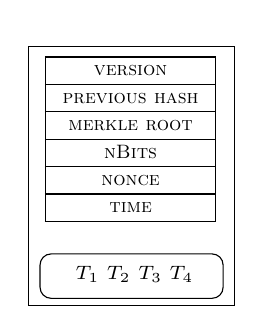
\begin{tikzpicture}[yscale=0.47,xscale=0.75]
   	\draw (0,0) rectangle (3.5,7);
   	\draw[rounded corners] (0.2,0.2) rectangle (3.3,1.4);
   	
   	\node[label,below] at(1.8,1.6) {\scriptsize $\Transaction_1$ $\Transaction_2$ $\Transaction_3$ $\Transaction_4$};
   	\node[label,below] at(1.8,7) {
	\begin{tabular}{|c|c|} \hline
              {\scriptsize \MName{version}}   		\\ \hline
	      {\scriptsize \MName{previous hash}} 	\\ \hline
              {\scriptsize \MName{merkle root}}  	\\ \hline
              {\scriptsize \MName{nBits}} 		\\ \hline
              {\scriptsize \MName{nonce}} 		\\ \hline
              {\scriptsize \MName{time}}  		\\ \hline
	\end{tabular}
	};
 
   \end{tikzpicture}
   \caption{A Bitcoin-style block containing a header and a body with transactions ($\Transaction_1$, $\Transaction_2$, $\Transaction_3$ and $\Transaction_4$).}
   \label{fig:block-structure}
\end{figure}

\section{Background: Proof-of-Work Consensus}
The {\em settlement} phase in our \DualChain{} architecture makes use of 
our novel \PoC{} protocol. The intuition behind \PoC's design stems from the 
\PoW{} protocol that helps create an immutable {\em chain of blocks}. The term 
immutable refers to the fact that each block appended to the chain requires miners 
to spend their resources. As a result, if an adversary attempts to over-write 
(or rollback) a part of the chain, it needs to create an alternate chain of all the 
desired blocks. However, to force all the honest miners to switch to this alternate 
chain, the adversary needs to compute this chain of blocks at a much faster rate 
than the original chain. This implies that the adversary needs to have much greater 
power than the honest miners. Prior works have illustrated that such an attack is 
hard to realize~\cite{bc-processing}.

Prior to running the \PoW{} protocol, each miner $\Miner \in \Miners$ needs to 
create a {\em block} of transactions. Although each miner $\Miner$ has access to the 
certificate $\Certificate$, it needs to arrange the contents of this certificate in 
the format of a block. To explain the format of a block, we follow the popular 
blockchain platform, Bitcoin, where each block includes a header and body 
(refer to Figure~\ref{fig:block-structure})~\cite{blockchain-book}. 
The header includes: 
(i) {\em version} for this block, 
(ii) {\em hash} of the previous block, 
(iii) {\em merkle root} of all transactions, 
(iv) {\em nBits}, which determines the difficulty of the puzzle, 
(v) {\em nonce}, the solution for puzzle, and 
(vi) {\em time} at which block is created once the nonce is found.

Computing Merkle root of all the transactions is trivial (refer to 
Figure~\ref{fig:merkle-tree}) and requires a miner $\Miner$ to compute a pairwise 
hash from the leaf to the root. This Merkle root helps to verify if a transaction 
was included to create the Merkle tree. However, the main challenge for a miner is 
to determine the nonce. In existing \PoW{}-based platforms, to solve the complex 
puzzle, each miner needs to calculate the {\em hash of the block} such that it 
contains a specific number of leading zero bits. For this purpose, the miners have 
to find a {\em nonce} value that yields the specific hash. This essentially makes the 
\PoW{} protocol like a {\em race} where all the miners are competing against each 
other to find the nonce. Whichever miner finds a valid nonce first, it gets the chance 
to propose the next block to be added to the chain. Hence, coming up with the correct 
number of leading zero bits in the hash is important as it sets the difficulty of 
the puzzle which simplicity controls the average time taken for each winning miner 
to propose a block. Once a miner finds the valid nonce, it can fill all the entries 
in the header, and it broadcasts the new block to all the other miners.


\begin{figure}[t]\label{ex:merkle_tree}
       \centering
       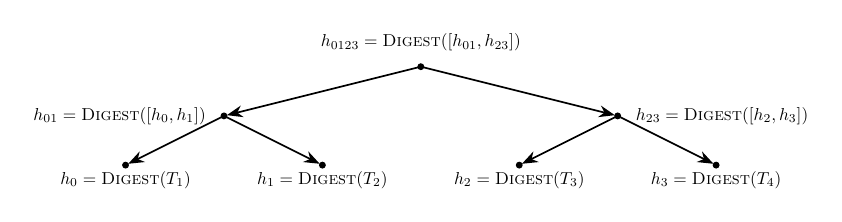
\begin{tikzpicture}[scale=0.625,transform shape]
           \node[dot] (n1) at (0, 0) {};
           \node[dot] (n2) at (4, 0) {};
           \node[dot] (n3) at (8, 0) {};
           \node[dot] (n4) at (12, 0) {};
           
           \node[below] at (n1) {$h_0 = \Digest{\Transaction_1}$};
           \node[below] at (n2) {$h_1 = \Digest{\Transaction_2}$};
           \node[below] at (n3) {$h_2 = \Digest{\Transaction_3}$};
           \node[below] at (n4) {$h_3 = \Digest{\Transaction_4}$};
   
           \node[dot] (n12) at (2, 1) {} edge[->] (n1) edge[->] (n2);
           \node[dot] (n34) at (10, 1) {} edge[->] (n3) edge[->] (n4);
   
           \node[left=7pt] at (n12) {$h_{01} = \Digest{[h_0, h_1]}$};
           \node[right=7pt] at (n34) {$h_{23} = \Digest{[h_2, h_3]}$};
   
           \node[dot] (n1234) at (6, 2) {} edge[->] (n12) edge[->] (n34);
        
           \node at (6,2.5) {$h_{0123} = \Digest{[h_{01},h_{23}]}$};
   
       \end{tikzpicture}
      	\caption{A Merkle tree over four transactions ($\Transaction_1$, $\Transaction_2$, 
      	$\Transaction_3$ and $\Transaction_4$) stored at the leaf nodes of the tree.}
	\label{fig:merkle-tree}
\end{figure} 


Notice that the ledger is essentially a chain of blocks (refer to Figure~\ref{fig:blockchain}).
In \PoW{}, it is possible that multiple miners propose the next block with valid 
nonces at approximately the same period of time. In such a case, the protocol states 
that each miner would only accept the first block it receives. This could lead to 
temporary branches or {\em forks}, all of which have the same previous hash. However, 
this condition resolves as time goes by because the protocol also expects the honest 
miners to stick to the {\em longest chain}\textemdash the one with the largest number 
of blocks. Eventually, all the shorter forks are discarded, and only the longest 
chain survives.

{\em Incentives.} 
Considering discarded forks and resources spent in the search for a valid nonce, 
what motivates a miner to participate in \PoW{} consensus? The answer is incentives. 
\PoW{}-based systems like Bitcoin reward the winning miner of the block present 
in the longest chain. These rewards help to offset the mining costs and maintain a  
sufficient number of honest miners. This requires a few more entries in the block header, 
which provide information such as the miner's account address and the reward amount.


\begin{figure}[t]
       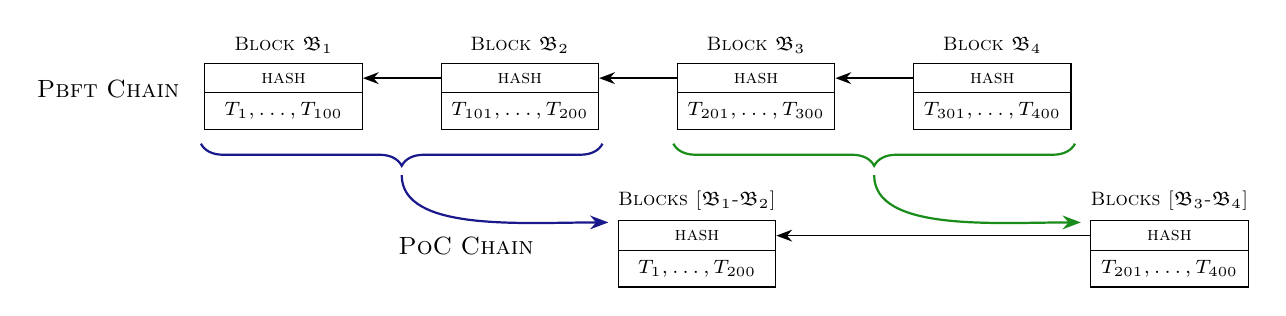
\begin{tikzpicture}[xscale=1.5,list/.style={minimum width=2cm,rectangle split, rectangle split parts=2,draw, rectangle split}]

           \node[list] (A) at (0, 0) {\scriptsize \MName{hash}\nodepart{two}\scriptsize \MName{$\Transaction_1, \dots, \Transaction_{100}$}};
           \node[list] (B) at (2, 0) {\scriptsize \MName{hash}\nodepart{two}\scriptsize \MName{$\Transaction_{101}, \dots, \Transaction_{200}$}};
           \node[list] (C) at (4, 0) {\scriptsize \MName{hash}\nodepart{two}\scriptsize \MName{$\Transaction_{201}, \dots, \Transaction_{300}$}};
           \node[list] (D) at (6, 0) {\scriptsize \MName{hash}\nodepart{two}\scriptsize \MName{$\Transaction_{301}, \dots, \Transaction_{400}$}};
           \node[above] at (A.north) {\scriptsize \MName{Block $\block_1$}};
           \node[above] at (B.north) {\scriptsize \MName{Block $\block_2$}};
           \node[above] at (C.north) {\scriptsize \MName{Block $\block_3$}};
           \node[above] at (D.north) {\scriptsize \MName{Block $\block_4$}};
           \path (D.text west) edge[->] (C.text east)
                 (C.text west) edge[->] (B.text east)
                 (B.text west) edge[->] (A.text east)
                 (A.text west);
                                         
\draw[decoration={brace,amplitude=8pt,mirror},decorate,thick,blue!50!black!90] (-0.7, -0.6) -- (2.7,-0.6);                 

\draw[decoration={brace,amplitude=8pt,mirror},decorate,thick,green!50!black!90] (3.3, -0.6) -- (6.7,-0.6);                 

\draw [->,thick, blue!50!black!90] (1,-1) to [out=270,in=180] (2.75,-1.6);
\draw [->,thick, green!50!black!90] (5,-1) to [out=270,in=180] (6.75,-1.6);
                 
                 
           \node[list] (E) at (3.5, -2) {\scriptsize \MName{hash}\nodepart{two}\scriptsize \MName{$\Transaction_{1}, \dots, \Transaction_{200}$}};
           \node[list] (F) at (7.5, -2) {\scriptsize \MName{hash}\nodepart{two}\scriptsize \MName{$\Transaction_{201}, \dots, \Transaction_{400}$}};
           \node[above] at (E.north) {\scriptsize \MName{Blocks [$\block_1$-$\block_2$]}};
           \node[above] at (F.north) {\scriptsize \MName{Blocks [$\block_3$-$\block_4$]}};
           \path (F.text west) edge[->] (E.text east);
           
\node[left] at (-0.8, 0.1) {{\small $\PBFT{}$ \MName{Chain}}};
\node[left] at (2.2, -1.9) {{\small $\PoC{}$ \MName{Chain}}};                            
                 
       \end{tikzpicture}
       \caption{A schematic representation of a blockchain or ledger in the 
       \DualChain{} architecture that consists of $\PBFT{}$ chain (i.e., \textit{layer 1}) 
       and $\PoC{}$ chain (i.e., \textit{layer 2}) that shows committed and settled 
       transactions $\Transaction_1, \dots, \Transaction_{400}$ on the $\PBFT{}$ and  
       $\PoC{}$ chains, respectively. The $i^{th}$ block holds a \emph{hash value} 
       hash$_{i-1}$ that identifies the preceding block and Block $\block_1$ is the  
       genesis block that does not have the preceding block.}
	\label{fig:blockchain}
\end{figure}



\subsection{\PoW{} Challenges}
The key issue with running the \PoW{} consensus is that it leads to massive 
waste in energy and efforts:
(1) Forks of the longest chain are subsequently discarded, which is a loss of 
resources for some miners who did find a valid nonce but did not receive any rewards.
(2) Rational miners may acquire more resources to improve their chances of proposing 
the next block, but this leads to increasing the difficulty of hash computation to 
ensure fairness.
(3) As the number of miners increases, the frequency of a single miner winning rewards 
decreases. 
(4) Several miners may work together in groups to find the valid nonce to increase 
their probability of winning rewards. This behavior significantly decreases the 
probability for a lone miner to propose the next block.
(5) Malicious miners may attempt to perform attacks like selfish mining and 
double-spending, which can rollback client transactions and invalidate the rewards earned 
by honest miners~\cite{blockchain-book}.

These issues are so prevalent in blockchain systems like Bitcoin that, 
at present, almost every miner is trying to join some existing group. In these 
groups, miners {\em pool} their resources to find a valid nonce and propose the 
next block~\cite{pooled-mining}. Every pool has its own participation rules and 
distributes rewards according to its policies. Despite this, the difficulty of hash 
computation is periodically increased or decreased in accordance with the average 
time to find a nonce by a pool of miners.

To address these challenges, in this paper, we aim to initiate a new avenue of research 
centered around hybrid consensus and collaborative mining. In particular, as a first step,
we propose our novel {\em Power-of-Collaboration} (\PoC) protocol that re-imagines 
the \PoW{} consensus.
\section{\DualChain{} Architecture}
\label{s:dual}
Our \DualChain{} runs two distinct consensus protocols in parallel. 
Specifically, it requires the replicas in set $\Replicas{}$ to commit each client transaction
through a \BFT{} consensus protocol (commitment phase), following which the miners in set $\Miners{}$ run our \PoC{} 
consensus (settlement protocol). As all the \BFT{} protocols follow the consensus dictated by 
\pbft~\cite{pbftj}, we use \pbft{} as the representative protocol 
for the ensuing discussions.
%
{\em To summarize:} each client sends its request to the replicas running the \pbft{} protocol. 
Once these replicas commit this request, they forward it to the miners. 
These miners collaboratively run the \PoC{} consensus protocol, post 
which they add a block to the ledger. Next, we discuss each of these steps 
in detail.

\begin{figure}[t]
   \centering
   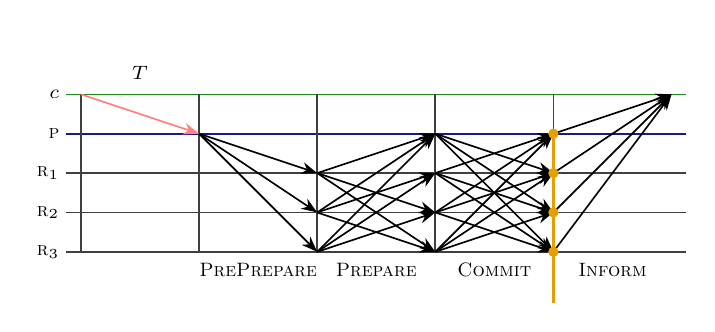
\begin{tikzpicture}[yscale=0.5,xscale=0.75]
       \draw[thick,draw=black!75] (1.75,   0) edge ++(10.5, 0)
                                  (1.75,   1) edge ++(10.5, 0)
                                  (1.75,   2) edge ++(10.5, 0)
                                  (1.75,   3) edge[blue!50!black!90] ++(10.5, 0)
                                  (1.75,   4) edge[green!50!black!90] ++(10.5, 0);

       \draw[thin,draw=black!75] (2, 0) edge ++(0, 4)
                                 (4,   0) edge ++(0, 4)
                                 (6, 0) edge ++(0, 4)
                                 (8,   0) edge ++(0, 4)
                                 (10,   0) edge ++(0, 4);

       \node[left] at (1.8, 0) {\scriptsize $\Replica_3$};
       \node[left] at (1.8, 1) {\scriptsize $\Replica_2$};
       \node[left] at (1.8, 2) {\scriptsize $\Replica_1$};
       \node[left] at (1.8, 3) {\scriptsize $\Primary{}$};
       \node[left] at (1.8, 4) {\scriptsize $\Client$};

       \path[->] (2, 4) edge [red!50](4, 3)
       
                 (4, 3) edge (6, 2)
                        edge (6, 1)
                        edge (6, 0)                        
                       
                 (6, 0) edge (8, 1)
                        edge (8, 2)
                        edge (8, 3)      
                
                 (6, 1) edge (8, 0)
                        edge (8, 2)
                        edge (8, 3)
                       
                 (6, 2) edge (8, 0)
                        edge (8, 1)
                        edge (8, 3)

                 (8, 0) edge (10, 1)
                        edge (10, 2)
                        edge (10, 3)
                       
                 (8, 1) edge (10, 0)
                        edge (10, 2)
                        edge (10, 3)
                       
                 (8, 2) edge (10, 0)
                        edge (10, 1)
                        edge (10, 3)
                       
                 (8, 3) edge (10, 0)
                        edge (10, 1)
                        edge (10, 2)
                 (10, 0) edge (12, 4)
                 (10, 1) edge (12, 4)
                 (10, 2) edge (12, 4)
                 (10, 3) edge (12, 4);
      
       \node[dot,colA] at (10, 0) {};
       \node[dot,colA] at (10, 1) {};
       \node[dot,colA] at (10, 2) {};
       \node[dot,colA] at (10, 3) {};
      
       \path (10, 3) edge[thick,colA] (10, -1.3);
       %\node[label,below right,align=left] at (10, 0) {\scriptsize \MName{Inform}};

       \node[label,below,yshift=3pt] at (3, 5) {\scriptsize \MName{$\Transaction$}};
       \node[label,below,yshift=3pt] at (5, 0) {\scriptsize \MName{PrePrepare}};
       \node[label,below,yshift=3pt] at (7, 0) {\scriptsize \MName{Prepare}};
       \node[label,below,yshift=3pt] at (9, 0) {\scriptsize \MName{Commit}};
       \node[label,below,yshift=3pt] at (11, 0) {\scriptsize \MName{Inform}};
   \end{tikzpicture}
   \caption{A schematic representation of the normal-case of the \pbft{} 
   protocol with $\n{\Replicas{}} = 4$ and $\f{\Replicas} = 1$. 
	%The primary $\Primary$ proposes a transaction $\Transaction{}$ submitted by client $\Client$ to all replicas via a $\MName{PrePrepare}$ message. Next, each replica broadcasts a $\MName{Prepare}$ message for $\T$. Upon a replica $\Replica$ receives $\NonFaulty_{pbft}$ for $\T$ from distinct replicas, $\Replica$ broadcasts a $\MName{Commit}$ message. Upon a replica $\Replica$ receives $\T$ from distinct replicas, execute $\T$ and inform $\Client$ the outcome.
	}
   \label{fig:pbft}
\end{figure}


\subsection{Client Request and Transaction Ordering}
\pbft{} follows the primary-backup model where one replica is designated as the 
{\em primary} while other replicas act as backups. Each consensus is led by the 
primary replica of the current {\em view}. In the case the primary is malicious, 
{\em view-change} takes place to replace the primary. We use Figure~\ref{fig:pbft} 
to illustrate the three phases of \pbft{}.


{\em Client Request.}
A client $\Client{}$ that wants to process a transaction $\Transaction{}$ in 
our \DualChain{} architecture creates a request $\SignMessage{\Transaction}{\Client{}}$ 
and sends it to the replica designated as the primary of the view $v$. The 
client $\Client{}$ uses \DS{} to sign this message and 
adds a monotonically increasing timestamp to this message.

{\em Pre-prepare.} 
When the primary $\Primary{}$ replica receives a well-formed client request 
$m := \SignMessage{\Transaction}{\Client{}}$, it assigns $m$ a sequence number 
$k$ and creates and sends a $\MName{Preprepare}$ message to all the replicas.
This $\MName{Preprepare}$ message also includes a digest $\Hash{m}$ of $m$, 
which is used in future communication to save space. During this phase, it is 
sufficient for the primary to sign the messages using \MAC{}.
%
When a replica $\Replica{} \in \Replicas{}$ receives a well-formed 
$\MName{Preprepare}$ message from the primary $\Primary{}$ of view $v$, it agrees 
to support the order $k$ for $m$ if it has not agreed to order another request 
at sequence number $k$. The replica $\Replica$ shows its support by broadcasting 
a $\MName{Prepare}$ message.

{\em Prepare.}
When a node $\Replica{}$ receives identical $\MName{Prepare}$ messages from 
$2\f{\Replicas{}}+1$ distinct replicas (can include its own message to reach the 
count), it marks the request $m$ as {\em prepared} and broadcasts a $\MName{Commit}$ 
message. In \DualChain, we require each replica $\Replica{}$ to use $\MName{DS}$ 
to sign the $\MName{Commit}$ message.

{\em Commit.}
When $\Replica{}$ receives identical $\MName{Commit}$ messages from 
$2\f{\Replicas{}}+1$ replicas, it marks $m$ as {\em committed}. If $\Replica{}$ 
has executed all requests with sequence number less than $k$, it executes $m$ and 
sends a $\MName{Response}$ message to the client, which includes the result of 
execution $r$. The client $\Client$ marks $\SignMessage{\Transaction}{\Client{}}$ 
as processed when it receives identical $\MName{Response}$ messages from at least 
$\f{\Replicas{}}+1$ replicas.

{\bf \em Chain Communication.} 
Post consensus on $m$, each replica $\Replica$ creates a certificate $\Certificate$, 
which includes: 
(i) the client request $m$,
(ii) $\MName{Commit}$ messages for $m$ from $2\f{\Replicas{}}+1$ replicas, and
(iii) the result $r$.
Next, the replicas may follow the {\em cluster-sending} protocol~\cite{byz-cluster-sending} 
or delayed replication protocol~\cite{delayedrepl} to communicate with the miners 
in set $\Miners$.\footnote{We can model chain communication as either push- or pull-based 
model using existing peer-to-peer communication primitives.} The cluster-sending 
protocol guarantees the delivery of at least one message between the two clusters, 
given that less than one-third of members of each cluster are malicious. To do so, 
each member from the sending cluster sends a message to a distinct member in the 
receiving member. In our case, we need the certificate $\Certificate$ to be sent to 
at least $2\f{\Miners}+1$ miners: replica $\Replica{1}$ sends $\Certificate$ to miner 
$\Miner_{1}$; replica $\Replica{2}$ sends $\Certificate$ to miner $\Miner_{2}$, and 
so on.


\begin{figure}[t]
   \centering
    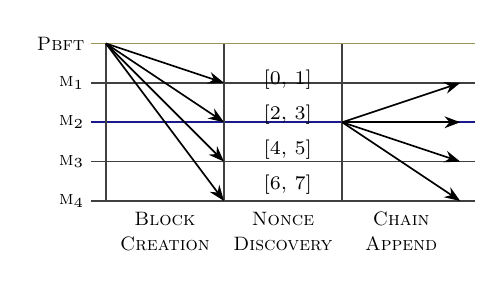
\begin{tikzpicture}[yscale=0.5,xscale=0.75]
           \draw[thick,draw=black!75] (1.75,   0) edge ++(6.5, 0)
                                   (1.75,   1) edge ++(6.5, 0)
                                   (1.75,   2) edge [blue!50!black!90] ++(6.5, 0)
                                   (1.75,   3) edge ++(6.5, 0)
                                   (1.75,   4) edge [yellow!50!black!90]++(6.5, 0);

           \node[label,below,yshift=3pt] at (3, 0) {\scriptsize \MName{Block}};
           \node[label,below,yshift=-6pt] at (3, 0) {\scriptsize \MName{Creation}};
           \node[label,below,yshift=3pt] at (5, 0) {\scriptsize \MName{Nonce}};
           \node[label,below,yshift=-6pt] at (5, 0) {\scriptsize \MName{Discovery}};
           \node[label,below,yshift=3pt] at (7, 0) {\scriptsize \MName{Chain}};
           \node[label,below,yshift=-6pt] at (7, 0) {\scriptsize \MName{Append}};
            
           \draw[thin,draw=black!75]   (2, 0) edge ++(0, 4)
                                       (4, 0) edge ++(0, 4)
                                       (6, 0) edge ++(0, 4);

           \node at (5, 1.8) {
                  \renewcommand{\arraystretch}{1.05}
           \begin{tabular}{c}
                  {\scriptsize[0, 1]}  \\
                  {\scriptsize[2, 3]}  \\
                  {\scriptsize[4, 5]}  \\
                  {\scriptsize[6, 7]}  \\
           \end{tabular}
           };

       \node[left] at (1.8, 0) {\scriptsize $\Miner_4$};
       \node[left] at (1.8, 1) {\scriptsize $\Miner_3$};
       \node[left] at (1.8, 2) {\scriptsize $\Miner_2$};
       \node[left] at (1.8, 3) {\scriptsize $\Miner_1$};
       \node[left] at (1.8, 4) {\scriptsize $\PBFT{}$};
       
       \path[->] (2, 4) 
                            edge (4, 3)                      
                            edge (4, 2)     
                            edge (4, 1)
                            edge (4, 0);
       \path[->] (6, 2) 
                            edge (8, 3)                      
                            edge (8, 2)
                            edge (8, 1)
                            edge (8, 0);

    \end{tikzpicture}
    	\caption{A schematic representation of the \PoC{} protocol with 
    	$\Miners{} = \{\Miner_1, \Miner_2, \Miner_3, \Miner_4\}$. 
    	The total solution space $\Slice{}$ is $[0,7]$ and is divided into four 
    	slices $([0,1], [2,3], [4,5], [6,7])$. Miners receive transactions from 
    	the \pbft{} replicas. Post creating a block, each Miner 
    	$\Miner_{i}$, $i \in [1,4]$ tries to discover the nonce in its slice 
    	$\Slice{i}$. Assume the valid nonce is $2$, then once $\Miner_2$ discovers 
    	the nonce, it broadcasts the same to other miners.
	}
	\label{fig:poc}
\end{figure}

When a miner $\Miner \in \Miners$ receives a certificate $\Certificate$ from 
a replica $\Replica \in \Replicas$, it broadcasts this certificate to all the 
other miners. As at least $2\f{\Miners}+1$ miners receive certificates, there 
is a guarantee that at least one honest miner will broadcast the certificate.
As a result, each miner will have access to the certificate $\Certificate$, and 
it can proceed with the \PoC{} computation.


\subsection{Collaborative Mining}
Post \pbft{} consensus, our \DualChain{} system runs the \PoC{} protocol on the 
agreed transaction to securely bind it to the ledger.
\PoC{} requires all the miners to {\em collaborate} and work together to compute 
the required hash. To do so, \PoC{} divides the \PoW{} hash computation into 
$\n{\Miners}$ disjoint subproblems and requires each miner to work on a distinct 
predetermined subproblem.

Let, $\Slice{}$ represent the solution space; all the random numbers that a miner 
has to try to find a valid nonce. Without the loss of generality, let us divide 
$\Slice{}$ into $\n{\Miners}$ equal slices, 
$\{ \Slice{1}, \Slice{2}, \cdots \Slice{\n{\Miners}} \}$, such that%

\begin{equation}
\Slice{1} \cap \Slice{2} \cap \cdots \cap \Slice{\n{\Miners}} = \varnothing 
\end{equation}%

\begin{equation}
\Slice{1} \cup \Slice{2} \cup \cdots \cup \Slice{\n{\Miners}} = \Slice{} 
\end{equation}

Our \PoC{} protocol assigns slice $\Slice{1}$ to miner $\Miner_{1}$, $\Slice{2}$ 
to $\Miner_{2}$, and $\Slice{i}$ to $\Miner_{i}$, $i \in [1,\n{\Miners}]$. The key 
assumption is that if a miner takes time $\tau$ to find a valid nonce on the solution 
space $\Slice{}$, then if all the miners are honest and follow the \PoC{} protocol, 
the time required to find the nonce should be of the order 
$\BigO{\dfrac{\tau}{\n{\Miners{}}}}$.

Further, \PoC{} protocol ensures that each honest miner gets rewarded for their 
efforts; rewards are distributed among miners. If $\Diamond$ is the reward for a 
miner to find a valid nonce in \PoW{} protocol, then in our \PoC{} protocol, each 
$i^{th}$ miner $\Miner_{i}$ receives a reward $\Diamond_i$ proportional to the size 
of its slice $\Slice{i}$.%

\begin{equation} 
    \Diamond_i = \frac{\abs{\Slice{i}}}{\abs{\Slice{}}} * \Diamond
\end{equation}

In the rest of this paper, for simplicity, we assume that all the slices have the same size.

\subsubsection{\PoC{} Protocol}
Our \PoC{} protocol works in rounds, and within each round each miner tries to find 
if a valid nonce exists in its slice of the block. In the rest of this section, we 
assume that the solution space $\Slice{}$ can be deterministically divided into 
$\n{\Miners{}}$ disjoint equal slices by each miner. For example, in Figure~\ref{fig:poc}, 
the solution space $\Slice{} = [0,7]$ is divided into $\n{\Miners{}} = 4$ slices; the 
slices are: $\Slice{1} = [0,1]$, $\Slice{2} = [2,3]$, $\Slice{3} = [4,5]$, and $\Slice{4} = [6,7]$.
Designing optimal slice distribution schemes is an interesting research avenue, which 
we consider outside the scope of this work.
%It contains two steps: obtain client transactions from $\PBFT{}$ network and mining the new block. We define the transactions in $\block_i$ mined in round i as $\TXNBlock_i$ and all $\TXNBlock_i$ are the same.

{\em Certificate Dissemination.} 
The \PoC{} protocol starts when a miner $\Miner{}$ receives a certificate $\Certificate$ 
from a replica. The miner $\Miner{}$ checks if $\Certificate$ is well-formed and 
$\Certificate$ includes signatures from $2\f{\Replicas{}}+1$ replicas; a proof that 
these replicas agreed to sequence this batch of transactions at a sequence number $k$.
If this is the case, $\Miner{}$ broadcasts this certificate to other miners.
Note: although while explaining \pbft{} we considered consensus on a single transaction, 
it can be trivially extended to a batch of transactions. This batching optimization is 
employed by all the existing \BFT{} protocols to increase their 
throughputs~\cite{pbftj,poe,rcc}.

{\em Block Creation.}
When a miner $\Miner$ has the nonce for the block ordered at sequence number $k-1$, 
it initiates the creation of a block at sequence $k$. It does so by generating a Merkle root 
of all the transactions in $k^{th}$ batch and a new block header. As each miner 
$\Miner{}$ knows there are a total of $\n{\Miners}$ miners, it creates $\n{\Miners}$ 
slices and assigns itself the $i^{th}$ slice $\Slice{i}$ in round $0$, where 
$i = \ID{\Miner{}}$.

{\em Nonce Discovery.}
We assume that each miner $\Miner{}$ knows the characteristics of the expected hash 
(the number of leading zeroes). The miner uses this information to go over all the 
possible nonces in its slice range to find a valid nonce. Once a miner $\Miner$ 
computes the correct hash, it has access to a valid nonce. The miner $\Miner$ uses 
this information to complete the block header and forwards the block to all the miners.

{\em Chain Append.}
When a miner receives a block from another miner, it first validates the nonce. If 
the nonce is valid, the miner appends this block to its local blockchain and assumes 
the \PoC{} protocol for the corresponding batch as complete.
% 
Notice that if all the miners are well-behaving, then our \PoC{} protocol requires 
only one round to find the valid nonce as the nonce is present in one of the slices.
Post discovering the nonce, each miner starts working on the next block to be added to 
the chain.

%\begin{figure}[t!]\label{ex:poc_no_solution}
%   \centering
%       \centering
%    \begin{tikzpicture}[yscale=0.5,xscale=0.75]
%           \draw[thick,draw=black!75] (0.75,   0) edge ++(14.5, 0)
%                                   (0.75,   1) edge ++(14.5, 0)
%                                   (0.75,   2) edge ++(14.5, 0)
%                                   (0.75,   3) edge ++(14.5, 0)
%                                   (0.75,   4) edge [yellow!50!black!90]++(14.5, 0);
%
%           \node[label,below,yshift=3pt] at (2, 0) {\scriptsize \MName{Block [$\block{1}$]}};
%           \node[label,below,yshift=3pt] at (4, 0) {\scriptsize \MName{Nonce}};
%           \node[label,below,yshift=-6pt] at (4, 0) {\scriptsize \MName{Discovery}};
%           \node[label,below,yshift=-15pt] at (4, 0) {\scriptsize \MName{(Timeout)}};
%           \node[label,below,yshift=3pt] at (6, 0) {\scriptsize \MName{Slice}};
%           \node[label,below,yshift=-6pt] at (6, 0) {\scriptsize \MName{Shift}};
%           \node[label,below,yshift=3pt] at (8, 0) {\scriptsize \MName{Nonce}};
%           \node[label,below,yshift=-6pt] at (8, 0) {\scriptsize \MName{Discovery}};
%           \node[label,below,yshift=-15pt] at (8, 0) {\scriptsize \MName{(Timeout)}};
%           \node[label,below,yshift=3pt] at (10, 0) {\scriptsize \MName{Block}};
%           \node[label,below,yshift=-6pt] at (10, 0) {\scriptsize \MName{[$\block{1}$, $\block{2}$]}};
%           \node[label,below,yshift=3pt] at (12, 0) {\scriptsize \MName{Nonce}};
%           \node[label,below,yshift=-6pt] at (12, 0) {\scriptsize \MName{Discovery}};
%           \node[label,below,yshift=3pt] at (14, 0) {\scriptsize \MName{Chain}};
%           \node[label,below,yshift=-6pt] at (14, 0) {\scriptsize \MName{Update}};
%            
%           \draw[thin,draw=black!75]   (1, 0) edge ++(0, 4)
%                                       (3, 0) edge ++(0, 4)
%                                       (5, 0) edge ++(0, 4)
%                                       (7, 0) edge ++(0, 4)
%                                       (9, 0) edge ++(0, 4)
%                                       (11, 0) edge ++(0, 4)
%                                       (13, 0) edge ++(0, 4.2);
%
%       \node[left] at (0.8, 0) {\scriptsize $\Miner_4$};
%       \node[left] at (0.8, 1) {\scriptsize $\Miner_3$};
%       \node[left] at (0.8, 2) {\scriptsize $\Miner_2$};
%       \node[left] at (0.8, 3) {\scriptsize $\Miner_1$};
%       \node[left] at (0.8, 4) {\scriptsize $\PBFT{}$};
%
%       \node at (4, 1.8) {
%                  \renewcommand{\arraystretch}{1.05}
%           \begin{tabular}{c}
%                  {\scriptsize \MName[0, 1]}  \\
%                  {\scriptsize \MName[2, 3]}  \\
%                  {\scriptsize \MName[4, 5]}  \\
%                  {\scriptsize \MName[6, 7]}  \\
%           \end{tabular}
%           };
%
%       \path[->] (1, 4) 
%                            edge (3, 3)                      
%                            edge (3, 2)     
%                            edge (3, 1)
%                            edge (3, 0);
%       \path[->] (5, 3) 
%                            edge (7, 3)                      
%                            edge (7, 2)     
%                            edge (7, 1)
%                            edge (7, 0);
%       \path[->] (5, 2) 
%                            edge (7, 3)                      
%                            edge (7, 2)     
%                            edge (7, 1)
%                            edge (7, 0);
%       \path[->] (5, 1) 
%                            edge (7, 3)                      
%                            edge (7, 2)     
%                            edge (7, 1)
%                            edge (7, 0);
%       \path[->] (5, 0) 
%                            edge (7, 3)                      
%                            edge (7, 2)     
%                            edge (7, 1)
%                            edge (7, 0);
%       \node at (8, 1.8) {
%                  \renewcommand{\arraystretch}{1.05}
%           \begin{tabular}{c}
%                  {\scriptsize \MName[2, 3]}  \\
%                  {\scriptsize \MName[4, 5]}  \\
%                  {\scriptsize \MName[6, 7]}  \\
%                  {\scriptsize \MName[0, 1]}  \\
%           \end{tabular}
%       };
%       \path[->] (9, 4) 
%                            edge (11, 3)                      
%                            edge (11, 2)     
%                            edge (11, 1)
%                            edge (11, 0);
%       \node at (12, 1.8) {
%                  \renewcommand{\arraystretch}{1.05}
%           \begin{tabular}{c}
%                  {\scriptsize \MName[0, 1]}  \\
%                  {\scriptsize \MName[2, 3]}  \\
%                  {\scriptsize \MName[4, 5]}  \\
%                  {\scriptsize \MName[6, 7]}  \\
%           \end{tabular}
%           };
%
%       \path[->] (13, 1) 
%                            edge (15, 3)                      
%                            edge (15, 2)     
%                            edge (15, 1)
%                            edge (15, 0);
%
%    \end{tikzpicture}
%    	\caption{An example that no valid nonce can be found for the new block. If the {\em timer} $\delta$ fires because no valid new block arrives,
%           a Slice Shifting will be triggered by sending a shift message <SHIFT, h, $\ShiftRound{i}$> to other miners. If a miner $\Miner{j}$ receives
%           $2\f{\Replicas}+1$ same shift messages from distinct miners, it starts its $\ShiftRound{i+1}$ by assigning its $\Slice{j}$ to $\Slice{j+1}$
%           and start to find the valid nonce in the new $\Slice{j}$. If no valid block has been found after $\f{\Miners{}}$ rounds, we can determine 
%           that there is no solution for this new block. The transactions $\Transaction{}$ in this block will be merged into the next block and skip the
%           current one. We assume nonce 3 is the valid value for the second block that contains $\block{1} and \block{2}$ in this example.
%           }
%\end{figure}\label{fig:poc_no_solution}

\begin{figure}
   \centering
    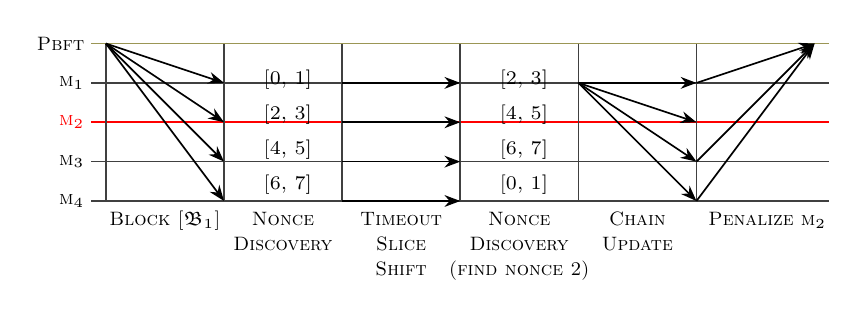
\begin{tikzpicture}[yscale=0.5,xscale=0.75]
           \draw[thick,draw=black!75] (0.75,   0) edge ++(12.5, 0)
                                   (0.75,   1) edge ++(12.5, 0)
                                   (0.75,   2) edge [red] ++(12.5, 0)
                                   (0.75,   3) edge ++(12.5, 0)
                                   (0.75,   4) edge [yellow!50!black!90]++(12.5, 0);

           \node[label,below,yshift=3pt] at (2, 0) {\scriptsize \MName{Block [$\block_{1}$]}};
           \node[label,below,yshift=3pt] at (4, 0) {\scriptsize \MName{Nonce}};
           \node[label,below,yshift=-6pt] at (4, 0) {\scriptsize \MName{Discovery}};
           \node[label,below,yshift=3pt] at (6, 0) {\scriptsize \MName{Timeout}};
           \node[label,below,yshift=-6pt] at (6, 0) {\scriptsize \MName{Slice}};
           \node[label,below,yshift=-15pt] at (6, 0) {\scriptsize \MName{Shift}};
           \node[label,below,yshift=3pt] at (8, 0) {\scriptsize \MName{Nonce}};
           \node[label,below,yshift=-6pt] at (8, 0) {\scriptsize \MName{Discovery}};
           \node[label,below,yshift=-15pt] at (8, 0) {\scriptsize \MName{(find nonce 2)}};
           \node[label,below,yshift=3pt] at (10, 0) {\scriptsize \MName{Chain}};
           \node[label,below,yshift=-6pt] at (10, 0) {\scriptsize \MName{Update}};
           \node[label,below,yshift=3pt] at (12.2, 0) {\scriptsize \MName{Penalize $\Miner_{2}$}};
            
           \draw[thin,draw=black!75]   (1, 0) edge ++(0, 4)
                                       (3, 0) edge ++(0, 4)
                                       (5, 0) edge ++(0, 4)
                                       (7, 0) edge ++(0, 4)
                                       (9, 0) edge ++(0, 4)
                                       (11, 0) edge ++(0, 4);
       \node[left] at (0.8, 0) {\scriptsize $\Miner_4$};
       \node[left] at (0.8, 1) {\scriptsize $\Miner_3$};
       \node[left,red] at (0.8, 2) {\scriptsize $\Miner_2$};
       \node[left] at (0.8, 3) {\scriptsize $\Miner_1$};
       \node[left] at (0.8, 4) {\scriptsize $\PBFT{}$};

       \node at (4, 1.8) {
                  \renewcommand{\arraystretch}{1.05}
           \begin{tabular}{c}
                  {\scriptsize \MName[0, 1]}  \\
                  {\scriptsize \MName[2, 3]}  \\
                  {\scriptsize \MName[4, 5]}  \\
                  {\scriptsize \MName[6, 7]}  \\
           \end{tabular}
           };

       \path[->] (1, 4) 
                            edge (3, 3)                      
                            edge (3, 2)     
                            edge (3, 1)
                            edge (3, 0);
       \path[->] (5, 3) 
                            edge (7, 3);
                            %edge (7, 2)     
                            %edge (7, 1)
                            %edge (7, 0);
       \path[->] (5, 2) 
                            %edge (7, 3)                      
                            edge (7, 2);     
                            %edge (7, 1)
                            %edge (7, 0);
       \path[->] (5, 1) 
                            %edge (7, 3)                      
                            %edge (7, 2)     
                            edge (7, 1);
                            %edge (7, 0);
       \path[->] (5, 0) 
                            %edge (7, 3)                      
                            %edge (7, 2)     
                            %edge (7, 1)
                            edge (7, 0);
       \node at (8, 1.8) {
                  \renewcommand{\arraystretch}{1.05}
           \begin{tabular}{c}
                  {\scriptsize \MName[2, 3]}  \\
                  {\scriptsize \MName[4, 5]}  \\
                  {\scriptsize \MName[6, 7]}  \\
                  {\scriptsize \MName[0, 1]}  \\
           \end{tabular}
       };
       \path[->] (9, 3) 
                            edge (11, 3)                      
                            edge (11, 2)     
                            edge (11, 1)
                            edge (11, 0);
       \path[->] (11, 3) 
                            edge (13, 4);
       \path[->] (11, 1) 
                            edge (13, 4);
       \path[->] (11, 0) 
                            edge (13, 4);

    \end{tikzpicture}
      \caption{An illustration of the slice shifting procedure. Here, we assume 
      $2$ is the valid nonce of the block, and the miner $\Miner_2$ is malicious. 
      Hence, $\Miner_2$ does not broadcast the block to other miners, which 
      triggers slice shifting procedure. Post slice shifting, $\Miner_1$ discovers 
      the nonce and broadcasts to other miners.
      }
	\label{fig:poc_malicious}
\end{figure}


\subsubsection{Slice Shifting Protocol}
In our \DualChain{} system, each miner receives certificates from the \pbft{} 
replicas. These certificates include client transactions that have been 
ordered by at least $2\f{\Replicas}+1$ replicas. Our \DualChain{} architecture 
uses the \PoC{} protocol to add these transactions to the ledger in the order 
defined by \pbft{} replicas. As a result, a malicious miner has limited attack 
opportunities; if a malicious miner finds a valid nonce in its slice, it can 
avoid forwarding this information to the honest miners. If such is the case, 
despite searching over its slice, each honest miner would not find any possible 
solution and would not be able to make progress.

To resolve this attack, our \PoC{} protocol requires each miner to set a 
{\em timer} $\delta$. Each miner $\Miner{}$ starts a timer $\delta$ when it 
receives a certificate from the \pbft{} replicas. $\Miner{}$ stops $\delta$ 
if it discovers the valid nonce or it receives a valid block from another miner.
If $\Miner{}$'s timer $\delta$ expires, and it does not have access to the valid 
nonce, it initiates the {\em slice shifting} protocol. Once the slice shifting 
is endorsed by the majority of miners, then each miner searches for the nonce 
in the next slice. Specifically, if prior to slice shifting a miner $\Miner{}$ 
was working on the $i^{th}$ slice $\Slice{i}$, post slice shifting $\Miner{}$ will 
work on $((i+1) \mod \n{\Miners{}})^{th}$ slice, $\Slice{(i+1)}$. As each miner 
already has access to all the slices, this switch does not require any 
additional communication.

The key intuition behind the slice shifting procedure is that even if a malicious 
miner decides to hide the nonce, post switch, it will be discovered by another miner.
However, it is possible that up to $\f{\Miners{}}$ consecutive miners may be malicious. 
As a result, the honest miners will discover the valid nonce after $\f{\Miners{}}$ shifts.%
\footnote{
The search space can be salted deterministically upon shifting to expand the search 
space and guard against rare cases in which the original problem may have no solution irrespective of minors' behavior.
}

%We impose all the solutions of $\PoW{}$ puzzles to be resolved in time T. (It is easy to restrict the solution time by modifying the difficulty, like Bitcoin estimate each block will be created average in 15 minutes and the longest mining time is no large than 2 hours from the median mining time of the previous 11 blocks[???]). 


\subsubsection{Reward and Penalty Economy}
Frequent slice shifting due to malicious miners will be detrimental to the 
performance of our \PoC{} protocol; it forces honest miners to do more work and 
wastes their resources. Moreover, why would any rational miner want to join the 
\PoC{} network and invest its computational resources? To make \PoC{} protocol 
fruitful, we incentivize all the honest miners for their efforts; all miners 
are assumed honest until proven guilty. 

First, like existing blockchain systems, such as Bitcoin and Ethereum, one of 
the aims of our \DualChain{} system is to establish a decentralized economy. 
To do so, like Bitcoin, in \PoC{}, when a miner discovers a nonce and broadcasts 
the valid block to other miners, we assume the creation of a {\em new token}. For 
brevity, we skip diving into the crypto-economics of the token generation and 
disbursement, and refer to the existing literature on the same~\cite{bitcoin,ether}. 
However, the key goal is that this token is equally divided among the honest 
miners. Further, like Bitcoin and Ethereum, we expect each client to pay some 
fees for getting its transaction processed by our \DualChain{} system. This 
fees is also equally divided among all the miners working on the current block.

To disburse transaction fees and tokens among the miners, there are two possible 
approaches: 
(i) Like Bitcoin, each miner includes $\n{\Miners{}}$ transactions that assigns an 
equal fraction of the reward to every other miner's public-key (account). These 
transactions can be deterministically created by each miner prior to mining and are 
included while creating the Merkle root. However, this will create unnecessary 
book-keeping, increasing the size of blocks.
(ii) We assume that the genesis block of the ledger records 
the information about the founding miners and their respective initial slices.
Further, miners can redistribute, resale, and divide their slices to other miners 
(similar to buying and selling of stocks), and any such transactions must be stored 
on the ledger before becoming effective. Assume that when a miner purchases a slice, 
sufficient tokens are reserved to enable penalization of misbehaving miners, 
which results in slashing their reserve funds similar to Proof-of-Stake 
designs~\cite{blockchain-book}. Given all this information, when a block is 
formed by the \PoC{} miners, we add the incentives to the accounts of
the respective miners; miners can validate if they received incentives or not. 

This rewarding process of \PoC{} is similar to strategies adopted by 
{\em mining pools} in systems like Bitcoin. Most importantly, in \PoC{}, the 
agreement on what to be included in the next block is strictly determined by \PBFT{} 
chain, not miners. This substantially simplifies the design of \PoC{} by making it 
deterministic, eliminating any lottery-based or leader-less consensus challenges 
that traditional \PoW{} must cope with. Furthermore, we present the novel idea of 
slice shifting for the cases when no miner in a round broadcasts a valid nonce. 
As slice shifting requires each miner to work on the next slice to find the nonce, 
it is expensive. We mitigate the need for slice shifting by heavily {\em penalizing} 
malicious miners. Specifically, we require each miner to count the number of 
{\em shifts} it took to find a valid nonce and to identify the miner who failed 
to find the valid nonce. Further, as the order of all initial slice assignments is known 
to all the miners, so each miner can trivially determine which miner was responsible 
for previous shifts. Notice that any misbehaving miner will be discovered and penalized 
as it diminishes the returns for other honest miners. 


%\begin{lemma}
%    If a non-faulty miner finds out the solution and broadcasts the new block in the ShiftRound $\ShiftRound{i}$, at least $2*\f{\Miners{}}+1$ miners will receive 
%    the new block in $\ShiftRound{i}$ if the following assumptions are ture [...].
%\end{lemma}


%We use pay-per-share(PPS)[???] as a reward stratery. Whenever a new block is created, every miner will receive the reward 
%according to their exploring solution space ($\Slice$). 
%


%Once a miner receives a new block in its shift round $\ShiftRound_i$, it believes that the solution owners on $[\ShiftRound_1 \cdots \ShiftRound_{i-1}$ are faulty 
%and should be punished, by sneding a new message <PENALIZE, Miners, height> via $\PBFT{}$ network where Miners are the faluty 
%minters who did not work on the solution in the previous shift round, heigh is the current block height. Once a replica in $\PBFT{}$ network
%receives $2*F^{\PoW{}}+1$ same penalty messages from different miners, send a <PENALIZE\_ACK,Miners,height> to the current primary.
%Once the current primary receives $2*F^{\PBFT{}}+1$ PENALIZE\_ACK messages from distinct replicas, submit the PENALIZE\_ACK message via a
%new transaction by $\PBFT{}$ consensus algorithm. This transaction will be executed by all the miners eventually thought $\PoC$ protocol.
%(Figure $\ref{fig:penalty_normal_case}$)
%
%If a replica in $\PBFT{}$ network sends out a PUSHNISH\_ACK to the primary but does not receive the commit message in some timeouts, it will re-send
%the messages. If the committed message still does not arrive after some retry, it will trigger a ViewChange to change the current primary 
%(Figure $\ref{fig:penalty_timeout}$). 
%
%\input{punishment_nc}

\section{Proof-of-Concept Evaluation}
We now present an initial evaluation of our vision of \DualChain{} architecture,
which we implement in the open-sourced \ResDB{} fabric~\cite{poe,geobft,rcc, 
ringbft}.\footnote{For our proof-of-concept of \DualChain{} 
architecture, we employ an experimental version of \ResDB{} with the codename of {\em NexRes} 
(Next Generation \ResDB{}); this is an architectural rewrite of the \ResDB{} 3.0 
(the latest stable version).}

\begin{figure*}
    \centering
    \setlength{\tabcolsep}{1pt}
    \begin{tabular}{cc@{\quad}cc}
        \pbfttput&
        \pbftlat\\
    \end{tabular}
    \vspace{-3mm}
    \caption{Evaluating peak throughput and commitment latency attained by \pbft{} consensus in \DualChain{}.}
    \vspace{-3mm}
    \label{fig:performance_pbft}
\end{figure*}

\begin{figure*}
    \centering
    \setlength{\tabcolsep}{1pt}
    \begin{tabular}{cc@{\quad}cc}
        \EvalBatchTput{(a)}&
        \EvalBatchLatency{(b)}&
        \EvalMinerTput{(c)}&
        \EvalMinerLatency{(d)}\\
    \end{tabular}
    \vspace{-3mm}
    \caption{Evaluating \PoC{} throughput and average settlement latency with 
    different difficulty (D), miners (M) and block batch size (B).}
    \vspace{-3mm}
    \label{fig:performance_poc}
\end{figure*}

{\bf Experimental Setup.}
We use Oracle Cloud Infrastructure's VM.Standard2.8 architecture to deploy miners 
and replicas ($16$ cores, \SI{8.2}{Gbps} bandwidth, $120$ GB Memory). In our 
experiments, we generate $400$ million client requests of size \SI{64}{B} each,
while client response has size \SI{17}{B}. We average results over three runs.
We require clients to sign their messages using \texttt{ED25519} while replicas use 
\texttt{CMAC}.

{\bf Batching.}
We employ the standard practice of batching client transactions, which we refer to 
\textit{transaction batching}, to optimize the \pbft{} consensus. Additionally, during 
the \PoC{} consensus, each miner aggregates multiple batches from \pbft{} consensus, '
which we refer to \textit{block batching}, prior to mining. 

 
{\bf \pbft{} Scaling.}
In Figure~\ref{fig:performance_pbft}, we gauge the peak throughput and 
\textit{commitment latency} incurred by the \pbft{} consensus of our \DualChain{} 
architecture. This is an important metric as it informs the rate at which we 
can reply to the clients. For this experiment, we increase the number of replicas 
from $16$ to $120$ and require the primary to process a batch of $100$ 
transactions per consensus; transaction batch size is set to $100$. 
As expected, on increasing the number of replicas, there is a drop in peak 
throughput and an increase in incurred latency, which remains in the subsecond 
range. This phenomenon occurs because, at each setting, we are approximately 
hitting the network bandwidth; as the number of replicas increases, more messages 
are communicated per consensus. In summary, the peak throughput reaches well 
over \SI{800}{k} transactions/second at $16$ replicas while sustaining over 
\SI{100}{k} transactions/second even when scaling to as many as $120$ replicas.


{\bf \PoC{} Scaling.}
Next, we study the impact of our \PoC{} consensus protocol on the \DualChain{} 
architecture. We deploy $120$ replicas for running \PBFT{} consensus. For the 
\PoC{} setting, we set the solution space parameter to $42$ nonce bits and 
split it into equal disjoint slices based on the number of miners. Notice that 
the difficulty of each problem is the number of leading zeros in the hash. In 
Figure~\ref{fig:performance_poc}, we present our results; here $D$ refers to 
difficulty (with the default of $D=9$), $M$ refers to the number of miners 
(with the default of $M=120$), and $B$ refers to the number of batches in a block. 
As stated earlier, for every $B$ blocks produced by \PBFT{} a single block is 
notarized and minted by \PoC{}.
 
In Figures~\ref{fig:performance_poc}(a) and~\ref{fig:performance_poc}(b), 
we fix the number of miners to $120$, which allows creating $120$ equal slices, and 
increase the block size from \SI{120}{k} to \SI{280}{k}. We test at two 
difficulty levels: $D=8$ and $D=9$. Our results indicate that $D=8$ is 
relatively easy, due to which each miner has to perform a smaller amount 
of work. As a result, any increase in batch size does not increase peak 
throughput. Hence, we test on $D=9$ at which mining smaller batch size 
impacts the system throughput as miners have to participate in a larger 
number of consensus rounds. On further increasing the block size, 
we observe that the throughput hits the \PBFT{}'s peak as desired. Thus, 
notarizing the blocks by \PoC{} no longer hinders the system throughput, 
it only prolongs the \textit{settlement latency} as expected. 
%
When examining the end-to-end system throughput of \DualChain{} which 
includes both \PBFT{} and \PoC{}, we observe a sustained throughput 
of \SI{105}{k} with a commitment latency of $1$ second and the settlement 
latency of $198$ seconds when the batch size is set to \SI{200}{k}. 
{\em Note:} We could not test at difficulty beyond $D=9$ as each nonce 
computation became prohibitively time- and resource-intensive given 
our available commodity hardware.

In Figures~\ref{fig:performance_poc}(c) and~\ref{fig:performance_poc}(d), 
we gauge the performance of \PoC{} when there are $64$ to $120$ miners. 
For these experiments, we also test at three different block batch sizes. 
As expected, the degree of collaborative mining is directly proportional 
to the number of miners. As we increase the number of miners, there is an
increase in peak throughput and a decrease in the settlement latency.


%In our experiments, we realize \mo{as expected not we realized} that when 
%the mining time is always smaller than the transaction producing time, 
%the miners will be always waiting for the transactions before they start 
%the \PoW{}. In this case, the \PoW{} throughput will be the same as the 
%\PBFT{} throughput. For example, it is much easier to find out the 
%solutions when we set the difficulty as eight. When we set up BBS larger 
%than 80K which will need 1.5 minute to fulfill in our \PBFT{} setting 
%but the mining latency is less than 1.5 minutes, the miners are idle 
%at most of the time. The throughput is consistence.  Thus, the throughput 
%will always be around (see  $\ref{fig:performance_poc}$). We also found 
%when we increase BBS to 120K, the throughput for difficulty nine will 
%also be around 100k. Due to the limitation of computation resource, 
%we are not able to evaluate the performance of difficulty ten.
%
%\mo{add the precise stats that justify our choice, for example, on 
%average solving puzzle with 9 leading zeros requires 3.724789943 minutes with 
%2 minutes standard deviation, which is why this block range make 
%sense} 
 

%\mo{for caption text, please see our earlier paper for more standard 
%formats.}

%\section{Related Work}
\label{sec:related-work}
\noindent \textbf{Pseudo-relevance feedback:} Our method has similarities with %the existing approach of 
Pseudo-Relevance Feedback (PRF) \cite{rocchio1971relevance, lv2009adaptive, li2022does} in IR: \cite{bendersky2011parameterized, xu2017quary} use the retrieved documents to improve sparse approaches via query expansion or query term reweighting, \cite{li2018nprf, zheng2020bert} score similarity between a target document and a top-ranked feedback document, while \cite{yu2021improving} train a separate query encoder that computes a new query embedding using the retrieved documents as additional input. In contrast, our approach does not require customized training feedback models or availability of explicit feedback data, as we improve the query vector by directly distilling from the reranker's output within an R\&R framework. %\pradeep{Why is our approach better?} 

Further, previous approaches to PRF have been dependent on the choice of retriever architecture and language; \cite{yu2021improving}'s PRF model is tied to the retriever used, \cite{chandradevan2022learning} explore cross-lingual relevance feedback, but require feedback documents in target language and thereby could only apply to three languages, while \cite{li2022interpolate} explore interpolating relevance feedback between dense and sparse approaches.
On the other hand, our approach is independent of the choice of the retriever and reranker architecture, and can be used for neural retrieval in any domain, language or modality. \\

\noindent \textbf{Distillation in Neural IR:} Existing approaches primarily leverage reranker feedback \textit{during training} of the dual-encoder retriever, to sample better negatives \cite{qu2021rocketqa}, for standard knowledge distillation of the cross-attention scores \cite{izacard2020distilling}, to train smaller and more efficient rankers by distilling larger models \cite{hofstatter2020improving}, or to align the geometry of dual-encoder embeddings with that from cross-encoders \cite{wang2021enhancing}. Instead, we leverage distillation at inference time, updating only the query representation to replicate the cross-encoder’s scores for the corresponding test instance.
A key implication of this design choice is that unlike existing methods, we keep the retriever parameters unchanged, meaning \textsc{ReFIT} can be incorporated out-of-the-box into any neural R\&R framework. In contrast, extending training-time distillation to new languages or modalities would require re-training the bi-encoder.

More recently, \textsc{TouR}~\cite{sung2023optimizing} has proposed test-time optimization of query representations with two variants: \textsc{TouR}$_{\text{hard}}$ and  \textsc{TouR}$_{\text{soft}}$. 
\textsc{TouR}$_{\text{hard}}$ optimizes the marginal likelihood of a small set of (pseudo) positive contexts.
\textsc{ReFIT} shares similarities with \textsc{TouR}$_{\text{soft}}$, which uses the normalized scores of a cross-encoder over the retrieved results as soft labels.
Crucially, \textsc{TouR} relies on multiple iterations of relevance feedback via distillation, where each iteration runs until the top-1 retrieval result has the highest reranker score (in \textsc{TouR}$_{\text{soft}}$) or is a pseudo-positive (in \textsc{TouR}$_{\text{hard}}$).
This makes inference highly computationally expensive, as each additional iteration involves labeling top-$K$ retrieval results with a reranker and then retrieving again.
\textsc{ReFIT} improves efficiency over \textsc{TouR} by requiring only a single iteration of feedback that simply updates the query vector for longer, foregoing additional retrieval and reranking steps. More specifics on the inference process of the two methods can be found in \S{\ref{sec:tour_comparison}}.
\textsc{TouR} was evaluated only on English phrase and passage retrieval tasks, while we demonstrate \textsc{ReFIT}'s effectiveness in multidomain, multilingual and multimodal settings, with an empirical comparison with \textsc{TouR} in \S{\ref{sec:tour_comparison}}.
\section{Conclusions}
In this paper, we present the vision of our \DualChain{} system, which facilitates 
the creation of a safe and efficient decentralized economy. \DualChain{} achieves these 
guarantees by separating the life-cycle of a client transaction into two phases: 
commitment and settlement. In the commitment phase, \DualChain{} employs a 
traditional \BFT{} protocol to order the client transactions. Post this, \DualChain{} 
requires a set of miners to run the settlement phase, where they notarize the ordered 
client transactions. Our \DualChain{} architecture does not impact the transaction 
latency observed by the client as each client receives the commitment response post 
\BFT{} consensus. Further, to efficiently notarize transactions during the settlement 
phase, our \DualChain{} architecture introduces the notion of collaborative mining, 
where participants work together instead of competing with each other. These notarized 
transactions are written to a ledger and can be queried in the future.


\section{Acknowledgments}
This work was supported in part by (1) {\em Oracle Cloud Credits} and 
related resources provided by the Oracle for Research program and (2) the 
{\em NSF STTR} under {\em Award Number} 2112345 provided to {\em Moka Blox LLC}.


%\balance
%\bibliographystyle{plain}
%\bibliography{submissions/junchao/refined}

\begin{thebibliography}{10}

\bibitem{sharper}
Mohammad~Javad Amiri, Divyakant Agrawal, and Amr El~Abbadi.
\newblock {\em {SharPer: Sharding Permissioned Blockchains Over Network
  Clusters}}, page 76–88.
\newblock Association for Computing Machinery, 2021.

\bibitem{bedrock}
Mohammad~Javad Amiri, Chenyuan Wu, Divyakant Agrawal, Amr~El Abbadi, Boon~Thau
  Loo, and Mohammad Sadoghi.
\newblock The bedrock of {BFT:} {A} unified platform for {BFT} protocol design
  and implementation.
\newblock {\em CoRR}, abs/2205.04534, 2022.

\bibitem{pbftj}
Miguel Castro and Barbara Liskov.
\newblock Practical byzantine fault tolerance and proactive recovery.
\newblock {\em ACM Trans. Comput. Syst.}, 20(4):398--461, 2002.

\bibitem{ahl}
Hung Dang, Tien Tuan~Anh Dinh, Dumitrel Loghin, Ee-Chien Chang, Qian Lin, and
  Beng~Chin Ooi.
\newblock Towards scaling blockchain systems via sharding.
\newblock In {\em Proceedings of the 2019 International Conference on
  Management of Data}, pages 123--140. ACM, 2019.

\bibitem{badcoin}
Alex de~Vries.
\newblock Bitcoin's growing energy problem.
\newblock {\em Joule}, 2(5):801--805, 2018.

\bibitem{sybil-attack}
John~R. Douceur.
\newblock The sybil attack.
\newblock In Peter Druschel, Frans Kaashoek, and Antony Rowstron, editors, {\em
  Peer-to-Peer Systems}, pages 251--260, Berlin, Heidelberg, 2002. Springer
  Berlin Heidelberg.

\bibitem{poe}
Suyash Gupta, Jelle Hellings, Sajjad Rahnama, and Mohammad Sadoghi.
\newblock {Proof-of-Execution}: Reaching consensus through fault-tolerant
  speculation.
\newblock In {\em Proceedings of the 24th International Conference on Extending
  Database Technology}, 2021.

\bibitem{blockchain-book}
Suyash Gupta, Jelle Hellings, and Mohammad Sadoghi.
\newblock {\em {Fault-Tolerant Distributed Transactions on Blockchain}}.
\newblock Synthesis Lectures on Data Management. Morgan {\&} Claypool
  Publishers, 2021.

\bibitem{rcc}
Suyash Gupta, Jelle Hellings, and Mohammad Sadoghi.
\newblock {RCC:} resilient concurrent consensus for high-throughput secure
  transaction processing.
\newblock In {\em 37th {IEEE} International Conference on Data Engineering,
  {ICDE} 2021, Chania, Greece, April 19-22, 2021}, pages 1392--1403. {IEEE},
  2021.

\bibitem{geobft}
Suyash Gupta, Sajjad Rahnama, Jelle Hellings, and Mohammad Sadoghi.
\newblock {ResilientDB}: Global scale resilient blockchain fabric.
\newblock {\em Proc. VLDB Endow.}, 13(6):868--883, 2020.

\bibitem{flexitrust}
Suyash Gupta, Sajjad Rahnama, Shubham Pandey, Natacha Crooks, and Mohammad
  Sadoghi.
\newblock Dissecting {BFT} consensus: In trusted components we trust!
\newblock {\em CoRR}, abs/2202.01354, 2022.

\bibitem{bc-processing}
Suyash Gupta and Mohammad Sadoghi.
\newblock Blockchain transaction processing.
\newblock In {\em Encyclopedia of Big Data Technologies}, pages 1--11.
  Springer, 2019.

\bibitem{byz-cluster-sending}
Jelle Hellings and Mohammad Sadoghi.
\newblock Brief announcement: The fault-tolerant cluster-sending problem.
\newblock In Jukka Suomela, editor, {\em 33rd International Symposium on
  Distributed Computing, {DISC} 2019}, volume 146 of {\em LIPIcs}, pages
  45:1--45:3, 2019.

\bibitem{delayedrepl}
Jelle Hellings and Mohammad Sadoghi.
\newblock Coordination-free byzantine replication with minimal communication
  costs.
\newblock In {\em 23rd International Conference on Database Theory, {ICDT}},
  pages 17:1--17:20, 2020.

\bibitem{cryptobook}
Jonathan Katz and Yehuda Lindell.
\newblock {\em Introduction to Modern Cryptography}.
\newblock Chapman and Hall/CRC, 2nd edition, 2014.

\bibitem{bitcoin}
Satoshi Nakamoto.
\newblock Bitcoin: A peer-to-peer electronic cash system, 2009.

\bibitem{ringbft}
Sajjad Rahnama, Suyash Gupta, Rohan Sogani, Dhruv Krishnan, and Mohammad
  Sadoghi.
\newblock {RingBFT: Resilient Consensus over Sharded Ring Topology}.
\newblock In {\em Proceedings of the 25th International Conference on Extending
  Database Technology}, pages 2:298--2:311. OpenProceedings.org, 2022.

\bibitem{pooled-mining}
Meni Rosenfeld.
\newblock Analysis of {Bitcoin} pooled mining reward systems, 2011.

\bibitem{mirbft}
Chrysoula Stathakopoulou, Matej Pavlovic, and Marko Vukolic.
\newblock State machine replication scalability made simple.
\newblock In Y{\'{e}}rom{-}David Bromberg, Anne{-}Marie Kermarrec, and Christos
  Kozyrakis, editors, {\em EuroSys '22: Seventeenth European Conference on
  Computer Systems}, pages 17--33. {ACM}, 2022.

\bibitem{basil}
Florian Suri-Payer, Matthew Burke, Zheng Wang, Yunhao Zhang, Lorenzo Alvisi,
  and Natacha Crooks.
\newblock Basil: Breaking up bft with acid (transactions).
\newblock In {\em Proceedings of the ACM SIGOPS 28th Symposium on Operating
  Systems Principles}, SOSP '21, page 1–17. Association for Computing
  Machinery, 2021.

\bibitem{badbadcoin}
Harald Vranken.
\newblock Sustainability of bitcoin and blockchains.
\newblock {\em Current Opinion in Environmental Sustainability}, 28:1--9, 2017.

\bibitem{ether}
Gavin Wood.
\newblock {Ethereum: A secure decentralised generalised transaction ledger}.
\newblock 2015.

\bibitem{hotstuff}
Maofan Yin, Dahlia Malkhi, Michael~K. Reiter, Guy~Golan Gueta, and Ittai
  Abraham.
\newblock {HotStuff}: {BFT} consensus with linearity and responsiveness.
\newblock In {\em Proceedings of the ACM Symposium on Principles of Distributed
  Computing}, pages 347--356. ACM, 2019.

\bibitem{scalable-ledger}
Kaiwen Zhang and Hans-Arno Jacobsen.
\newblock Towards dependable, scalable, and pervasive distributed ledgers with
  blockchains.
\newblock In {\em 2018 IEEE 38th International Conference on Distributed
  Computing Systems (ICDCS)}, pages 1337--1346, 2018.

\end{thebibliography}

\end{document}




